\chapter{Implementación del sistema de detección y reconocimiento de placas}
\label{ch:solucion}

\section{Generación sintética de imágenes}

La red neuronal end-to-end tiene la desventaja de requerir grandes cantidades de datos
para conseguir resultados con bajo error de entrenamiento y generalización;
habitualmente en el rango de 10 mil - 50 mil fotografías. 
En el tiempo disponible para la ejecución del proyecto no es posible 
capturar y etiquetar tal cantidad, además el costo de etiqueta de datos es 
elevado. El problema se mitiga utilizando imágenes sintéticas;
incrementando el conjunto de datos disponibles. 
Tales imágenes son creadas con base a la caracterización de las placas reales
y la fuente tipográfica usada en las mismas.

El conjunto artificial es utilizado para entrenar el modelo,
mientras que el conjunto de placas auténticas es usado
para la evaluación del sistema. Con ello se puede evaluar, indirectamente,
la utilidad de la estrategia, y la representatividad con la que conjunto sintético
asemeja al conjunto real en sus características esenciales.

En Costa Rica a las placas vehiculares se les asigna un código según el tipo de vehículos.
El reglamento sobre placas vehiculares especifica los códigos existentes, así como el color
del fondo de la placa y el color de los caracteres \cite{art97placasvehiculares}. Hay
más de 100 tipos de placas distintas.
Automóviles con códigos atípicos como el de placas extranjeras son poco probables de ser evaluadas;
además en el conjunto de imágenes reales no hay muestras de todos los tipos de placas.
Por este motivo solo se sintetizan placas basadas en las existentes en el conjunto de datos real
y las demás se dejan como casos no cubiertos o casos extremos. Los casos a cubrir se
muestran en la tabla \ref{tab:combinaciones-placas},
y sus características en \ref{tab:caracteristicas-placas}.

\begin{table}[H]
	\centering
	\begin{tabular}{|c|c|}
		\hline
			Tipo & Combinación \\
		\hline
			Particular & NNNNNN \\
		\hline
			Particular & LLL-NNN \\
		\hline
			TEC & 256 | NN \\
		\hline
			TEC & 256 | NNN \\
		\hline
			Carga ligera & CL | NNNNNN \\
		\hline
			Discapacitado & D-NNN \\
		\hline
			Motocicleta & M NNNNNN \\
		\hline
			Motocicleta & M $\frac{\text{NNN}}{\text{NNN}}$ \\
		\hline
	\end{tabular}
	\caption{Posible combinaciones de caracteres en placas costarricenses.}
	\label{tab:combinaciones-placas}
\end{table}

\begin{table}[H]
	\centering
	\begin{tabular}{|c|c|c|}
		\hline
			Código & Color placas & Color caracteres \\
		\hline
			 & Blanco & Azul \\
		\hline
			256 & Blanco & Verde \\
		\hline
			CL & Blanco & Rojo \\
		\hline
			 D & Blanco & Azul \\
		\hline
			 M & Blanco & Azul \\
		\hline
	\end{tabular}
	\caption{Características de placas costarricenses.}
	\label{tab:caracteristicas-placas}
\end{table}

Se producen los datos utilizando plantillas de placas reales y la fuente tipográfica real,
realizando recortes de los caracteres y dejando plantillas lo más limpias posibles.
Por ejemplo, las mostradas en Fig. \ref{fig:caracteres-full-azul} y \ref{fig:plantillas-full-blanco}.
Mediante software se crean placas aleatorias de forma sistemática,
tal como indica el diagrama de flujo \ref{fig:diagrama-flujo-generacion-multiples-placas}
y \ref{fig:diagrama-flujo-generador-placas}. 

\begin{figure}[H]
	\centering
	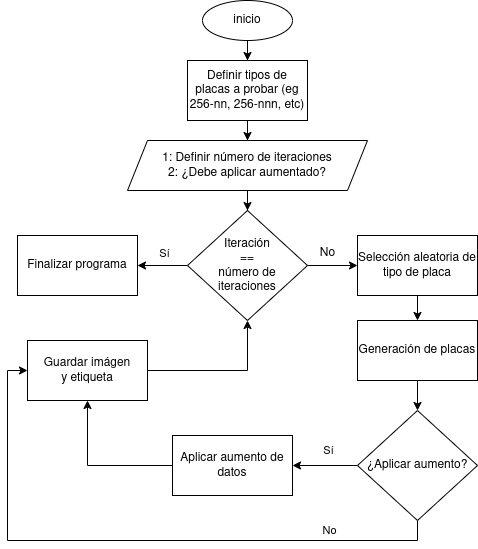
\includegraphics[width=\textwidth]{fig/proy/generacion-de-multiples-imagenes.drawio.png}
	\caption{Generación de múltiples imágenes sintéticas}
	\label{fig:diagrama-flujo-generacion-multiples-placas}
\end{figure}

\begin{figure}[H]
	\centering
	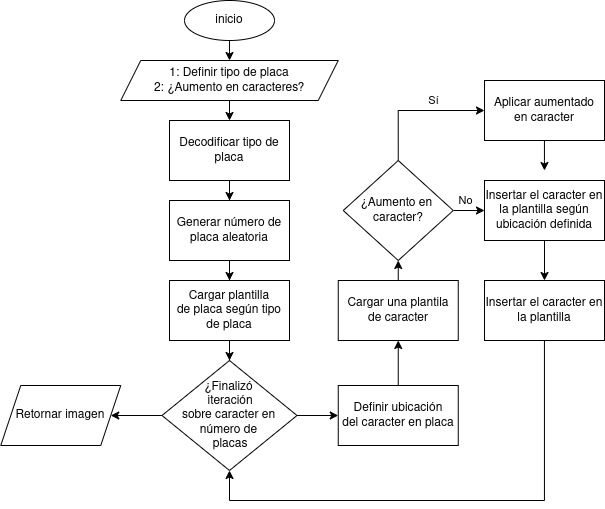
\includegraphics[width=\textwidth]{fig/proy/generacion-de-imagen-sintetica.drawio.png}
	\caption{Generación de imagen de placa sintética}
	\label{fig:diagrama-flujo-generador-placas}
\end{figure}

\section{Detección y extracción de ubicación de la placa en video e imágenes}

La detección de placas vehiculares en imágenes y video se realiza aplicando ajuste fino 
a modelos existentes. Se utiliza YOLOv11n.pt como principal, pues esta versión es 
más rápida y ofrece mejor capacidad de detección que sus predecesores. 
Se realiza además comparación de métricas con otras versiones de YOLO 
y con el modelo usado en el primer prototipo presentado en \cite{proyecto_previo}.

\section{Reconocimiento de número de placa}

